\univlogo

{\Huge March 28}\vspace{5mm}

\section*{Droop Control}


\subsection*{Power transmission of single inverter}

\begin{figure}[H]
\centering
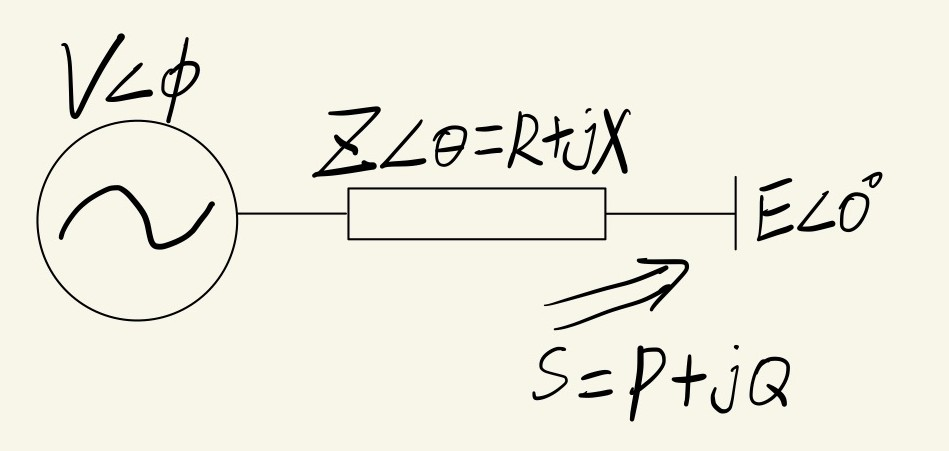
\includegraphics[width=0.6\textwidth]{./2023Mar/SingleInverter.png}
\caption{Single inverter}
\label{SingleInverter}
\end{figure}

\begin{equation}
\begin{aligned}
    S&=P+jQ=\dot{E}\dot{I}^* \\
    &=E\cdot \left (\cfrac{V\cos{\phi}+jV\sin{\phi}-E}{Z\cos{\theta}+jZ\sin{\theta}} \right )^*\\
    &=\cfrac{1}{Z}[(EV\cos{\phi}-E^2)\cos{\theta}+EV\sin{\phi}\sin{\theta}]\\
    &+j\cfrac{1}{Z}[(EV\cos{\phi}-E^2)\sin{\theta}-EV\sin{\phi}\cos{\theta}]
\end{aligned}
\end{equation}

So, the power is:

\href{run:./2023Mar/Derivation.jpg}{Derivation} 

\begin{equation}
\begin{aligned}
\left\{\begin{array}{l}
    P=(\cfrac{EV}{Z}\cos{\phi}-\cfrac{E^2}{Z})\cos{\theta}+\cfrac{EV}{Z}\sin{\phi}\sin{\theta}    \\
    Q=(\cfrac{EV}{Z}\cos{\phi}-\cfrac{E^2}{Z})\sin{\theta}-\cfrac{EV}{Z}\sin{\phi}\cos{\theta}
\end{array}\right.
\end{aligned}
\end{equation}

\subsection*{High terminal impedance transmission line}

When the terminal impedance of the inverter $R \gg X$, $X$ is neglected, at this time $\theta$ is treated as \textbf{0 (purely resistive circuit)}, and the voltage phase angle $\phi$ does not differ much from 0, $\sin{\phi}=\phi$, $\cos{\phi}=1$. The formula can be simplified to:

\begin{equation}
\begin{aligned}
\left\{\begin{array}{l}
    P \doteq \cfrac{E}{R}(V-E)    \\
    Q \doteq -\cfrac{EV}{R}\phi
\end{array}\right.
\end{aligned}
\end{equation}

\subsection*{High voltage transmission line}

When the transmission line is a high voltage line, $X \gg R$, at this time $\theta$ is treated as \textbf{$\cfrac{\pi}{2}$ (purely inductive circuit)}, and the voltage phase angle $\phi$ is relatively small, $\sin{\phi}=\phi$, $\cos{\phi}=1$. The formula can be simplified to:

\begin{equation}
\begin{aligned}
\left\{\begin{array}{l}
    P \doteq \cfrac{EV}{X}\phi    \\
    Q \doteq \cfrac{E}{X}(V-E)
\end{array}\right.
\end{aligned}
\end{equation}

It is clear that we can modify $P$ by changing the phase $\phi$, which is the integration of $\omega$, and Q is related to V.

Usually, the voltage angular frequency of the inverter is easier to monitor than the phase angle difference, so the droop control formula can be obtained by substituting the angular frequency for the phase angle difference:

\begin{equation}
\begin{aligned}
\left\{\begin{array}{l}
    \omega = \omega_0-m_pP    \\
    V = V_0 - n_qQ
\end{array}\right.
\end{aligned}
\end{equation}

If $P$ grows larger, $\omega$ becomes smaller.


